\chapter{Simulation\label{chap:simul}}
\textit{This chapter is somewhat technical, and can be skipped by readers
 uninterested in building and evaluating simulation systems.}
 \bigskip

I'd love to be able to ask questions like, ``how often does team A win against
  team B when team A subs out their lead?''
  and ``how does burning both shields on the lead affect chances of victory?''
I'd like to be able to take two teams and walk the game tree, seeing how
  each decision shapes future possible outcomes: ``There are 80 billion
  possible games from this point. If decision D is made, Team A
  wins 60\% of the remaining 60 billion. If decision E is made instead,
  Team A wins 80\% of the remaining 20 billion.'' Etc.

It is unlikely that simple closed form solutions exist describing
 the set of reasonable games between two arbitrary opponents (see \autoref{chap:unbounded}),
 let alone two teams.
For the highest level of predictive power, we must turn to machine-aided simulation.
Here we are lucky, for unlike most contests, Pokémon GO is concretely finite and discrete.
Its time evolves in half-second turns, each of which presents a small number of choices
  to both Trainers.
The use of random numbers is minimal.
Finally, it never diverges, instead advancing always towards a conclusion\footnote{There
  is an exception to convergence: both Trainers continuously choosing to do nothing (remember,
  even zero power attacks do one point of damage). This is pathological, and we
  simply dismiss all choice-pairs that change no state beyond the clock, neatly sidestepping this issue.
  Even if we didn't, there's a time limit on matches.}.

\section{Probabilistic methods\label{sec:probsimul}}
The easiest approach is similar to Monte Carlo integration.
At each turn, we evaluate the space of possibilities, and select one action for each Trainer.
This selection might be informed by an expert system, or take the form of a Markov chain,
 or combine these approaches.
Either way, each run takes exactly one path through the game tree, concluding with a single result.
This process is repeated many times, with more repetitions required for more
 diverse paths through the game tree\footnote{A pure expert system merits only
 one run---it generates the same path every time. As the number of
 probabilistic choices increases, so must the number of runs.}.
The output is an estimate of victory for each team (and ties).
This method is used by \href{https://pvpoke.com}{PvPoke} and, so far as I'm aware,
 all other simulation engines.
Runs are perfectly parallel, and trivially implemented in $\mathcal{O}(N)$ time
 and $\mathcal{O}(1)$ space on $N$ turns.

It has some shortcomings.
The results will only ever be as good as the model.
To the degree the model fails to reflect reality (i.e.\ when Trainers act outside
 its expectations), so will its predictions.
With that said, the ``right'' choice for a Trainer typically seems obvious,
 and easily described with a few simple rules.
They can likely be made quite accurate (widespread use by the community speaks to their predictive power).
Ideally, the output would be constantly evaluated against real battle results.
Automatic use of feedback would cause predictions to reflect the play of random Trainers,
 which might be undesirable (I presume an expert system would attempt to play like, well, an expert).
Still, \textit{without comparison against real results, we cannot meaningfully speak of the validity of predictions}.
Furthermore, questions like those earlier in this chapter become harder to answer,
 as we have less knowledge of paths considered unlikely by our model,
 and it is unlikely to bring unorthodox, new strategies to light.

\section{Exhaustive methods\label{sec:exhaustive}}
A naive solution begins at the first turn, generates the set of possible
  choices for both Trainers, and recurses across the Cartesian product
  of these sets: depth-first generation of the full game tree.
For each state, we must preserve the HP and energy of six Pokémon,
  the attack and defense buff level for two Pokémon,
  the number of turns remaining in two ongoing fast attacks,
  the number of shields remaining for each Trainer,
  and the turns remaining on each Trainer's substitution timer.
When done, we'll know how each choice affects the universe of possible outcomes,
  and how the teams ought fare for random choices.
Growth is clearly exponential: $\mathcal{O}(C^N)$ time for Cartesian products of size $C$ over $N$ turns.
Still, let's not reject exhaustive simulation out of hand.

What choices are available on a given turn?
If either Trainer has no Pokémon remaining, the match is over, and no choice
  need be made---we have our result, and can roll up our recursion.
A Trainer otherwise has between one and three Pokémon, one of which is active
  in the arena.
If the active Pokémon is in the middle of a multiturn fast attack, the
  Trainer has no choice to make.
Otherwise, if the substitution timer is inactive, the Trainer may sub in some other Pokémon.
If there is sufficient energy, the Trainer may call for a charged attack.
The Trainer can call for a fast attack, or do nothing for the turn.
In combination with these choices, a shield might or might not be used in response to a charged attack.
Each option must be pursued for an exhaustive search.

In the best case, each Trainer is waiting for an attack to complete.
In the worst case, each has ten choices, for a Cartesian product of 100 choicepairs---we
  blow up to ten billion states in five turns, and will not be going to space today.
This is $\mathcal{O}(100^N)$ time and $\mathcal{O}(N)$ state for $N$ turns.
We'll need prune the game tree using limited expert methods\footnote{We remain exhaustive, rather than
 stochastic, just within a limited space.}.

\subsection{Common state\label{subsec:commonstate}}
Whatever our method, implementing the trainer battle mechanics requires a
  three-vector for each team pointing into our (readonly) database of Pokémon and attacks.
\texttt{results} is shared across all nodes (and will need be protected should we go parallel).
Context in \texttt{simulstate} is duplicated each time we recurse; we need keep it tight.
\inputminted{cpp}{s/simul.h}

\section{Simulating 1x1\label{sec:simul1x1}}
Let's start with exhaustive simulation of a 1x1 contest,
 where substitution is not in play.
A naive implementation blows up almost immediately: the Trainer can choose to do nothing
 whenever they're not busy, and doing nothing consumes only one turn,
 meaning we almost always have at least four choicepairs:
 \{ noop, noop \}, \{ noop, fast \}, \{ fast, noop \}, and \{ fast, fast \}.
Our first restriction, then: there's no good reason to do nothing,
 so the Pokémon must do something.
On every turn, we either wait for our fast attack to conclude, or can throw a fast attack (\texttt{MOVE\_FAST}).
With sufficient energy, charged attacks enter the picture (\texttt{MOVE\_CHARGED1}, \texttt{MOVE\_CHARGED2}).
While we won't be implementing them yet, assuming other Pokémon have not
  fainted and the cooldown period is not active, we can substitute (\texttt{MOVE\_SUB1}, \texttt{MOVE\_SUB2}).
``One'' and ``two down'' here are taken modulo 3, i.e.\ if the third Pokémon is
  active, the first Pokémon is one down, and the second Pokémon is two down.
\inputminted{cpp}{s/moves.h}
Each turn is implemented in two halves.
The top half dispatches possible moves, determining choices available to
 the first player and invoking the appropriate inner half for each---it is our primary fan-out.
We need a function to determine which moves are viable for a Trainer on a given turn:
 \texttt{sift\_choices()} sets bits of a mask high if they're allowed\footnote{This minimizes
  code complexity, but we end up with twice the necessary branches, since the dispatched
  code varies wildly depending on the move type; these aren't exactly array indexes.
  Eh, let the branch predictor worry about that.}.
Should we reach for task parallelism, these loops are obvious targets.
\inputminted{cpp}{s/sift.h}
The inner half performs additional fan-out for charged attacks.
Each charged attack can break into shielded and unshielded paths.
Furthermore, we must simulate both paths in the event of a CMP tie---the tiebreaker
 might be nondeterministic, but we are not!
The result of \texttt{p0\_wins\_cmp()} is constant across a pair of Pokémon;
 we could cache it in the simulation state, recomputing on substitution or knockout.
The bottom half is invoked along each path, using its own copy of the state.
\inputminted{cpp}{s/bottom.h}
On a knockout, the top half calls \texttt{handle\_ko()}.
This is the only function that actually records results, and its loops are opportunities for further parallelism.
Right now we're only handling a single Pokémon per team, but we
 go ahead and implement this so that it'll work properly
 with arbitrarily many Pokémon.
When a Pokémon goes down, three things can happen:
\begin{itemize}
  \item No more Pokémon: the match is over.
  \item One more Pokémon: it becomes active. Continue the simulation.
  \item Two more Pokémon: simulate both replacements.
\end{itemize}
\inputminted{cpp}{s/ko.h}
The presented code simulates all possible meaningful exchanges of two fully specified Pokémon, starting
  with full HP, two shields, and no energy.

\lstinputlisting[basicstyle=\scriptsize]{output.lst}

\subsection{Closed forms in the endgame\label{subsec:endgame}}
Game simulation is friendly to memoization, i.e.\ storing and recognizing equivalent game states.
The easiest place to apply this is the endgame.
More correctly, this is the easiest way to choose states to memoize,
  such that we can efficiently look them up without blowing up memory.
Even better would be a closed form analytic treatment of the endgame,
  which seems like it ought be possible.
Let's restrict ourselves to the case of one Pokémon remaining per Trainer.
We dispense with charged attacks entirely (at least initially) by considering
  only those states where the possible turns remaining times EPT plus
  energy is less than the energy required for a charged attack.
This restriction means we can ignore shields, as they're only relevant
  when charged attacks are used.
We call these subgraphs ``death marches''.

How do we put an upper bound on turns?

\[ T_{max} = \min \left\lceil\frac{HP_1}{D_2}\right\rceil T_2,\left\lceil\frac{HP_2}{D_1}\right\rceil T_1 \]

$D$ is the damage inflicted per fast attack, and $T$ is the number of turns per fast attack.
This equation is well-defined for all attacks, since damage (unlike power,
  which can be zero) is always at least 1.
So, knowing $T_{max}$, we can determine those cases where no charged attack
  can be used: whenever $T_{max} * EPT + E_{current} < E_{charged}$ for both Pokémon.
There is only one possible path through such a subtree, with one answer:
  whichever Pokémon has a lower $T$ wins.

\section{Simulating 3x3\label{sec:simul3x3}}
Simulating a full Trainer Battle requires supporting three Pokémon per Trainer,
  simulating replacement paths when a Pokémon faints,
  and handling substitutions.
The increase in state is negligible, but substitutions have substantial impact on time complexity,
  since they can happen on any turn (unless there has been a recent substitution).
It furthermore represents two branches early, when a team has all three Pokémon.
Our death march closed form cannot be applied when a Pokémon remains.
Handling replacement is easier: all we need do is amend our frontend to
  seed all three positions, and implement switchover.
\vfill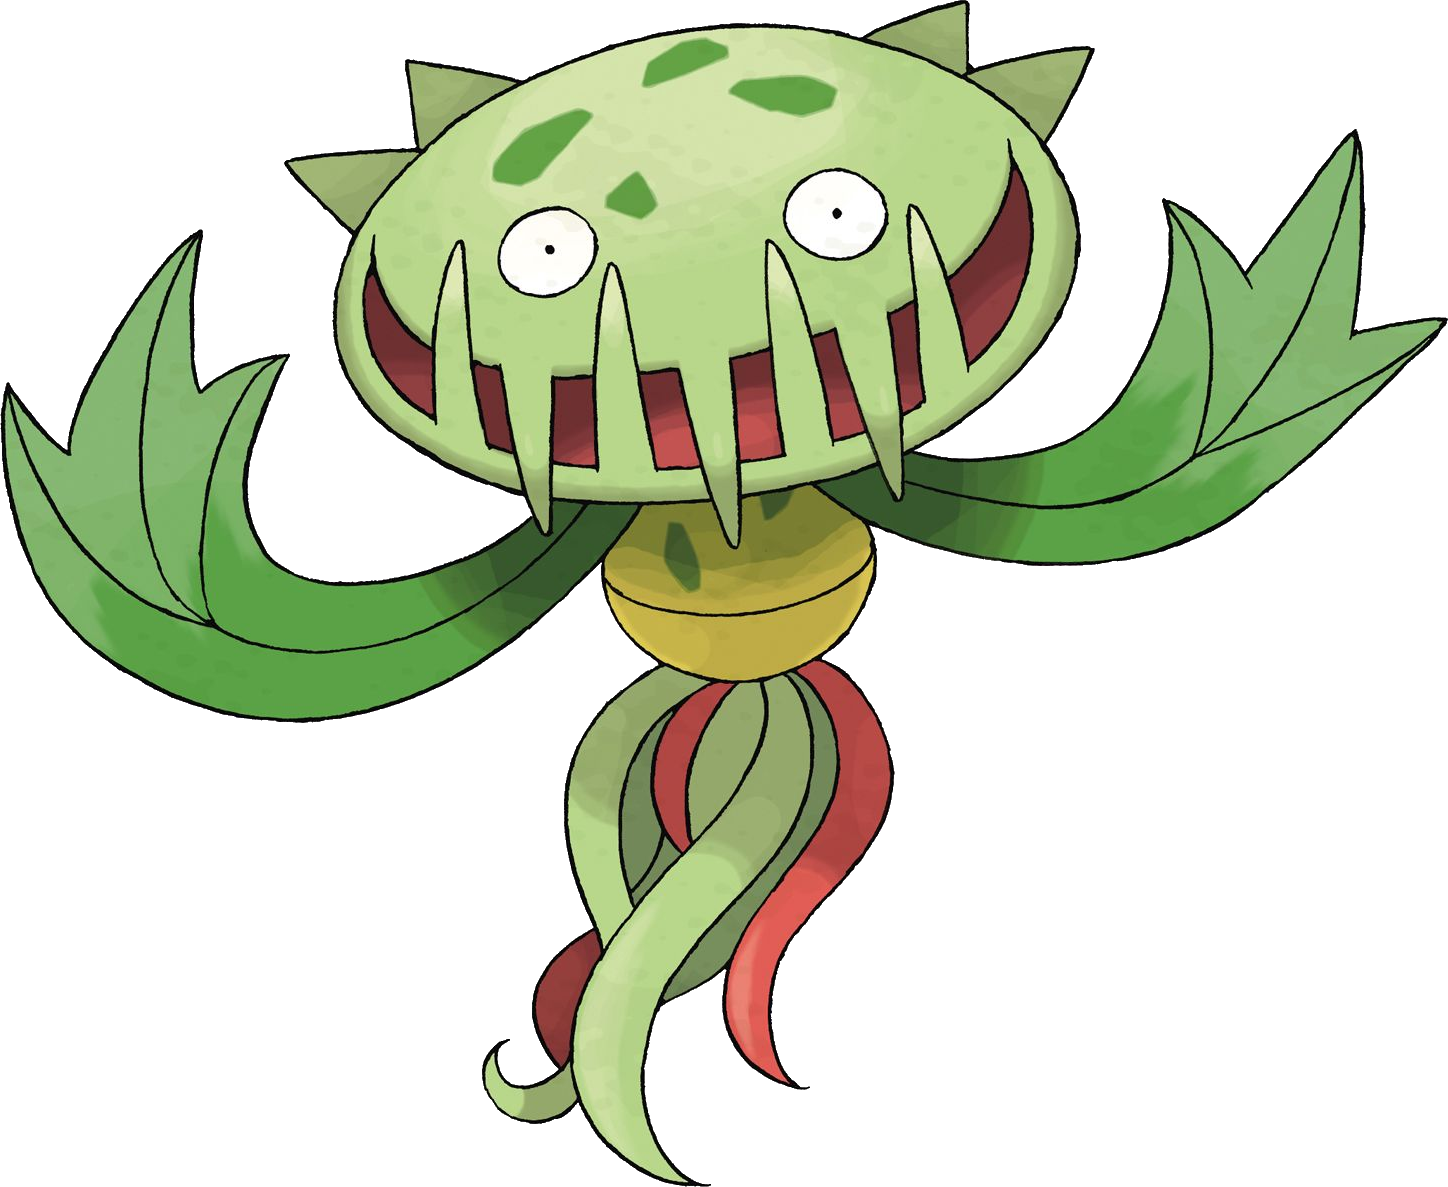
\includegraphics[width=\linewidth,keepaspectratio]{images/carnivine.png}
